
%$$$$$$$$$$$$$$$$$$$$$$$$$$$$$$$$$$$$$$$$$$$$$$$$$$$$$$$$$$$$$$$$$$$$$$$$$$$$$$$$
%Paragraph 2:Concurrent updates에 대한 연구
%$$$$$$$$$$$$$$$$$$$$$$$$$$$$$$$$$$$$$$$$$$$$$$$$$$$$$$$$$$$$$$$$$$$$$$$$$$$$$$$$
\newpage
\section{확장성 있는 자료구조 연구}
\label{sec:datarelated}
%Many scalable data structures with scalable schemes show different performances
% depending on their update ratios.
많은 확장성 있는 방법과 사용되는 자료구조들은 업데이트 비율에 따라 다른 성능을 가진다.  
%In low and middle update rate, researchers have attempted to create new
% scalable schemes~\cite{McKenney98}~\cite{Matveev2015RLU}~\cite{Harris2001Lockfree}
%~\cite{Fomitchev2004Lockfree}
%~\cite{Timnat2012}
%or have attempted to adapt these scheme to data
%structures~\cite{Arbel2014ConcurrentRCU}~\cite{Dodds2015SCT}~\cite{AustinTClements2012RCUBalancedTrees}.
낮거나 중간 정도의 업데이트 비율에서는 연구자들은 새로운 확장성있는
기법~\cite{McKenney98}~\cite{Matveev2015RLU}~\cite{Harris2001Lockfree} ~\cite{Fomitchev2004Lockfree}
~\cite{Timnat2012}을 연구하거나 그 기법을 자료구조에 
적용~\cite{Arbel2014ConcurrentRCU}~\cite{Dodds2015SCT}~\cite{AustinTClements2012RCUBalancedTrees}을
하도록 시도하고 있다.
%In high update rate, the OpLog shows significant improvement in
%performance scalability for update-heavy data structures in
%many core systems, but suffers from limitation and overhead due
%to time-stamp counter management.
높은 업데이트 비율에서는 OpLog가 매니코어의 업데이트 비율이 높은 자료 구조에 대해서
 상당히 높은 성능 확장성을 가진다. 
%We substantially extend our preliminary work~\cite{Kyong2016LDU} not only to
% support per-core algorithm but also to apply the \LDU to anonymous rmap due to improving the
%Linux kernel scalability.

\subsection{확장성 있는 자료구조를 위한 동기화 기법}

\subsubsection{RCU}


확장성을 위한 대표적 동기화 기법인 RCU는 McKenney와 Slingwine에 의해 개발되었고, 동기화 기법 때문에 발생하는 오버헤드를
최소화 시킨 방법이다.
특히 RCU는 리더들을 보호하기 위해 사용하는 동기화 기법의 오버헤드를 최소화 시킨다.
단점으로는 RCU의 라이터가 가 수행하는 방법은 복잡하고 느리다. 
이러한 단점에도 불구하고 리더들이 수행하는 락의 오버헤드가 적고, 여러 리더와 
업데이터 하나가 동시에 수행이 가능하므로 RCU는 현재 리눅스 커널에서 상당히 많이 사용되고 있다. 


\begin{figure}[h]
    \centering
    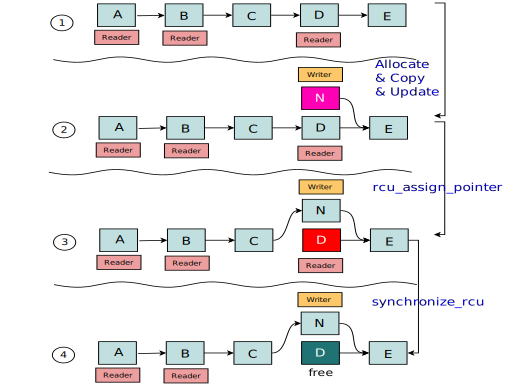
\includegraphics[width=1\textwidth]{fig/rcu/rcu_principle}
    \caption{RCU 예제}
  \label{fig:rcuprinciple}
\end{figure}

%$$$$$$$$$$$$$$$$$$$$$$$$$$$$$$$$$$$$$$$$$$$$$$$$$$$$$$$$$$$$$$$$$$$$$$$$$$$$$$$$
%Paragraph : RCU의 기본 철학
%$$$$$$$$$$$$$$$$$$$$$$$$$$$$$$$$$$$$$$$$$$$$$$$$$$$$$$$$$$$$$$$$$$$$$$$$$$$$$$$$
RCU의 기본 철학은 특정 시점에서 오브젝트를 복제해서 처리한다. 그림~\ref{fig:rcuprinciple}은 
이러한 RCU의 예를 보여준다.
그림에서 1단계에는 A, B, C, D, E 오브젝트 중 A, B, D 오브젝트를 리더들이 읽는 과정을 보여준다.
만약 이 순간 D 오브젝트를 수정하려 하면, RCU는 복사본을 할당 받고, 새로운 값인 오브젝트 N으로 수정을 한다.
그리고 다음 단계에서는 atomic한 연산을 통해서 오브젝트 C와 N을 연결한다. 
이 순간 오브젝트 D를 읽고 이는 리더와 다른 리더들은 아무런 블락 없이 계속 읽기를 수행할 수 있으며,
 동시에 업데이트까지 수행할 수 있어서 성능이 향상된다.
마지막으로 \code{synchroinze\_rcu()} 함수를 통해 리더가 읽기를 마칠 때 까지 기다리고, 읽기가 끝나면 
바로 \code{free()}를 수행한다. 
이 때 마지막 리더가 읽을 때 까지 기다리는 시간을 RCU에서는 grace period라 부른다. 

%$$$$$$$$$$$$$$$$$$$$$$$$$$$$$$$$$$$$$$$$$$$$$$$$$$$$$$$$$$$$$$$$$$$$$$$$$$$$$$$$
%Paragraph : RCU는 기본적으로 3가지 특징
%$$$$$$$$$$$$$$$$$$$$$$$$$$$$$$$$$$$$$$$$$$$$$$$$$$$$$$$$$$$$$$$$$$$$$$$$$$$$$$$$
RCU는 기본적으로 3가지 특징을 가진다. 첫 번째로 Lock-free 리더이다.
실제로 RCU의 리더들은 아무런 락 또는 배리어(barrier)를 소유하지 않고 수행되며, 리드 구간에서는
 per-core 자료구조에 단순히 enter/exit를 기록하여 수행한다. 
따라서, 락 발생하는 캐시 일관성 트래픽이 발생하지 않는다.
두번 째로, Single pointer update이다.
RCU의 writer는 atomic 명령으로 one pointer 업데이트를 수행한다.
이러한 특징으로 인해 여러 리더들과 한가지 업데이터가 동시에 동작할 수 있다.  
마지막으로, RCU는 delayed free를 수행한다.
노드를 바로 free를 하지 않고, 모든 리더들이 리드 구역을 벋어난 경우 까지 
기다린 후 해당 노드를 free한다.
이를 통해 안전하게 노드를 자원 해재할 수 있다. 

\begin{figure}[h]
    \centering
    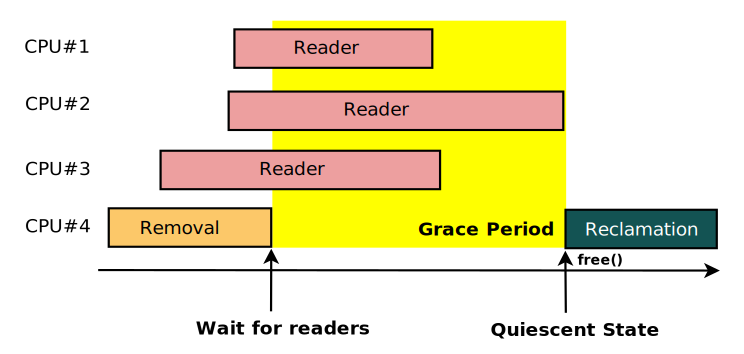
\includegraphics[width=1\textwidth]{fig/rcu/rcu_grace}
    \caption{RCU의 delayed free의 시점}
  \label{fig:rcu_grace}
\end{figure}

그림~\ref{fig:rcu_grace}는 RCU의 delayed free의 시점을 보여준다 . 


%$$$$$$$$$$$$$$$$$$$$$$$$$$$$$$$$$$$$$$$$$$$$$$$$$$$$$$$$$$$$$$$$$$$$$$$$$$$$$$$$
%Paragraph 2: RCU의 grace periad
%$$$$$$$$$$$$$$$$$$$$$$$$$$$$$$$$$$$$$$$$$$$$$$$$$$$$$$$$$$$$$$$$$$$$$$$$$$$$$$$$
RCU는 기본적으로 3가지 특징을 가진다. 첫 번째로 Lock-free 리더이다.
실제로 RCU의 리더들은 아무런 락 또는 배리어(barrier)를 소유하지 않고 수행되며, 리드 구간에서는
 per-core 자료구조에 단순히 enter/exit를 기록하여 수행한다. 
따라서, 락 발생하는 캐시 일관성 트래픽이 발생하지 않는다.
두번 째로, Single pointer update이다.
RCU의 writer는 atomic 명령으로 one pointer 업데이트를 수행한다.
이러한 특징으로 인해 여러 리더들과 한가지 업데이터가 동시에 동작할 수 있다.  
마지막으로, RCU는 delayed free를 수행한다.
노드를 바로 free를 하지 않고, 모든 리더들이 리드 구역을 벋어난 경우 까지 
기다린 후 해당 노드를 free한다.
이를 통해 안전하게 노드를 자원 해재할 수 있다. 

\begin{figure*}[h]
\begin{center}
\inputminted[linenos,fontsize=\footnotesize,
tabsize=4]{c}{src/rcu_list_data.c}
\end{center}
\caption{LDU의 동시적 삽제에 대한 알고리즘.}
\label{fig:gldulogicalupdate}
\end{figure*}



\begin{figure}[h!]
\begin{center}
\inputminted[linenos,fontsize=\footnotesize,
tabsize=4]{c}{src/rcu_list_search.c}
\end{center}
\caption{LDU의 동시적 삽제에 대한 알고리즘.}
\label{fig:gldulogicalupdate}
\end{figure}


\begin{figure}[h!]
\begin{center}
\inputminted[linenos,fontsize=\footnotesize,
tabsize=4]{c}{src/rcu_list_delete.c}
\end{center}
\caption{LDU의 동시적 삽제에 대한 알고리즘.}
\label{fig:gldulogicalupdate}
\end{figure}


%$$$$$$$$$$$$$$$$$$$$$$$$$$$$$$$$$$$$$$$$$$$$$$$$$$$$$$$$$$$$$$$$$$$$$$$$$$$$$$$$
%Paragraph 2: RCU의 예제 source 코드
%$$$$$$$$$$$$$$$$$$$$$$$$$$$$$$$$$$$$$$$$$$$$$$$$$$$$$$$$$$$$$$$$$$$$$$$$$$$$$$$$
RCU는 기본적으로 3가지 특징을 가진다. 첫 번째로 Lock-free 리더이다.
실제로 RCU의 리더들은 아무런 락 또는 배리어(barrier)를 소유하지 않고 수행되며, 리드 구간에서는
 per-core 자료구조에 단순히 enter/exit를 기록하여 수행한다. 
따라서, 락 발생하는 캐시 일관성 트래픽이 발생하지 않는다.
두번 째로, Single pointer update이다.
RCU의 writer는 atomic 명령으로 one pointer 업데이트를 수행한다.
이러한 특징으로 인해 여러 리더들과 한가지 업데이터가 동시에 동작할 수 있다.  
마지막으로, RCU는 delayed free를 수행한다.
노드를 바로 free를 하지 않고, 모든 리더들이 리드 구역을 벋어난 경우 까지 
기다린 후 해당 노드를 free한다.
이를 통해 안전하게 노드를 자원 해재할 수 있다. 



\subsubsection{RLU}

%$$$$$$$$$$$$$$$$$$$$$$$$$$$$$$$$$$$$$$$$$$$$$$$$$$$$$$$$$$$$$$$$$$$$$$$$$$$$$$$$
%Paragraph : RLU가 해결하고자 하는 문제
%$$$$$$$$$$$$$$$$$$$$$$$$$$$$$$$$$$$$$$$$$$$$$$$$$$$$$$$$$$$$$$$$$$$$$$$$$$$$$$$$
RLU는 \ldots
RCU는 기본적으로 3가지 특징을 가진다. 첫 번째로 Lock-free 리더이다.
실제로 RCU의 리더들은 아무런 락 또는 배리어(barrier)를 소유하지 않고 수행되며, 리드 구간에서는
 per-core 자료구조에 단순히 enter/exit를 기록하여 수행한다. 
따라서, 락 발생하는 캐시 일관성 트래픽이 발생하지 않는다.
두번 째로, Single pointer update이다.
RCU의 writer는 atomic 명령으로 one pointer 업데이트를 수행한다.
이러한 특징으로 인해 여러 리더들과 한가지 업데이터가 동시에 동작할 수 있다.  
마지막으로, RCU는 delayed free를 수행한다.
노드를 바로 free를 하지 않고, 모든 리더들이 리드 구역을 벋어난 경우 까지 
기다린 후 해당 노드를 free한다.
이를 통해 안전하게 노드를 자원 해재할 수 있다. 


%$$$$$$$$$$$$$$$$$$$$$$$$$$$$$$$$$$$$$$$$$$$$$$$$$$$$$$$$$$$$$$$$$$$$$$$$$$$$$$$$
%Paragraph : RLU가 해결한 방법
%$$$$$$$$$$$$$$$$$$$$$$$$$$$$$$$$$$$$$$$$$$$$$$$$$$$$$$$$$$$$$$$$$$$$$$$$$$$$$$$$
RCU는 기본적으로 3가지 특징을 가진다. 첫 번째로 Lock-free 리더이다.
실제로 RCU의 리더들은 아무런 락 또는 배리어(barrier)를 소유하지 않고 수행되며, 리드 구간에서는
 per-core 자료구조에 단순히 enter/exit를 기록하여 수행한다. 
따라서, 락 발생하는 캐시 일관성 트래픽이 발생하지 않는다.
두번 째로, Single pointer update이다.
RCU의 writer는 atomic 명령으로 one pointer 업데이트를 수행한다.
이러한 특징으로 인해 여러 리더들과 한가지 업데이터가 동시에 동작할 수 있다.  
마지막으로, RCU는 delayed free를 수행한다.
노드를 바로 free를 하지 않고, 모든 리더들이 리드 구역을 벋어난 경우 까지 
기다린 후 해당 노드를 free한다.
이를 통해 안전하게 노드를 자원 해재할 수 있다. 


\subsubsection{Non-locking synchronization}



%$$$$$$$$$$$$$$$$$$$$$$$$$$$$$$$$$$$$$$$$$$$$$$$$$$$$$$$$$$$$$$$$$$$$$$$$$$$$$$$$
%Paragraph : Non-locking synchronization의 장점
%$$$$$$$$$$$$$$$$$$$$$$$$$$$$$$$$$$$$$$$$$$$$$$$$$$$$$$$$$$$$$$$$$$$$$$$$$$$$$$$$
Non-blocking synchronization은 장점은 여러 스레드들이 락 기반으로 자원을 관리함에 따라
 발생하는 문제를 해결할 수 있다. 
가장 큰 장점은 스레드 또는 프로세스가 락 때문에 기다리는 시간을 제거할 수 있다.
이 것은 락을 얻기 위해 기다리는 시간을 최소화 할 뿐만 아니라 무한 루프 때문에 무한정 기다리는 
데드락 같은 상황까지 제거 할 수 있다. 
다음으로 모든 락은 락 자체의 오버헤드를 가지고 있는데 이것을 제거할 수 있다. 
예를 들어 코어 수가 증가 할 수록 락 자체를 얻기 위해 원자적 명령을 이용한느데 이것은 캐시 일관성 트래픽을 
발생한다. 
이와 같이 Non-blocking 방법은 이러한 락 자체가 가지고 있는 문제점인 데드락(deadlock), 라이브락(livelock), 
우선순위 역전현상(priority inversion)등을 제거 할 수 있다. 

이러한 Non-blocking synchronization 기법을 사용하는 lock-free 자료 구조들은 성능을 향상 시킬 수 있다. 
그 이유는 멀티코어 환경에서 공유되는 데이터를 접근하기 위해 직렬화 되는 부분이 매우 짧기 때문이다. 

\begin{figure}[h!]
    \centering
    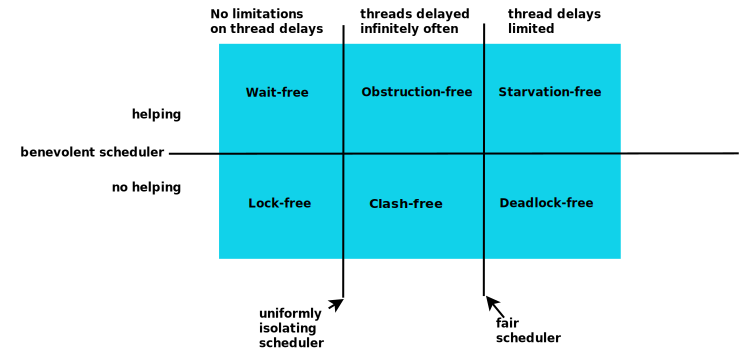
\includegraphics[width=1\textwidth]{fig/NBS/NBS}
    \caption{Non-locking synchronization}
  \label{fig:NBS}
\end{figure}


%$$$$$$$$$$$$$$$$$$$$$$$$$$$$$$$$$$$$$$$$$$$$$$$$$$$$$$$$$$$$$$$$$$$$$$$$$$$$$$$$
%Paragraph : Non-locking synchronization 알고리즘 종류 1 
%$$$$$$$$$$$$$$$$$$$$$$$$$$$$$$$$$$$$$$$$$$$$$$$$$$$$$$$$$$$$$$$$$$$$$$$$$$$$$$$$
Non-blocking synchronization은 장점은 여러 스레드들이 락 기반으로 자원을 관리함에 따라
 발생하는 문제를 해결할 수 있다. 
가장 큰 장점은 스레드 또는 프로세스가 락 때문에 기다리는 시간을 제거할 수 있다.
이 것은 락을 얻기 위해 기다리는 시간을 최소화 할 뿐만 아니라 무한 루프 때문에 무한정 기다리는 
데드락 같은 상황까지 제거 할 수 있다. 
다음으로 모든 락은 락 자체의 오버헤드를 가지고 있는데 이것을 제거할 수 있다. 
예를 들어 코어 수가 증가 할 수록 락 자체를 얻기 위해 원자적 명령을 이용한느데 이것은 캐시 일관성 트래픽을 
발생한다. 
이와 같이 Non-blocking 방법은 이러한 락 자체가 가지고 있는 문제점인 데드락(deadlock), 라이브락(livelock), 
우선순위 역전현상(priority inversion)등을 제거 할 수 있다. 
이러한 Non-blocking synchronization 기법을 사용하는 lock-free 자료 구조들은 성능을 향상 시킬 수 있다. 
그 이유는 멀티코어 환경에서 공유되는 데이터를 접근하기 위해 직렬화 되는 부분이 매우 짧기 때문이다. 


%$$$$$$$$$$$$$$$$$$$$$$$$$$$$$$$$$$$$$$$$$$$$$$$$$$$$$$$$$$$$$$$$$$$$$$$$$$$$$$$$
%Paragraph :  Non-locking synchronization 알고리즘 종류 2
%$$$$$$$$$$$$$$$$$$$$$$$$$$$$$$$$$$$$$$$$$$$$$$$$$$$$$$$$$$$$$$$$$$$$$$$$$$$$$$$$
Non-blocking synchronization은 장점은 여러 스레드들이 락 기반으로 자원을 관리함에 따라
 발생하는 문제를 해결할 수 있다. 
가장 큰 장점은 스레드 또는 프로세스가 락 때문에 기다리는 시간을 제거할 수 있다.
이 것은 락을 얻기 위해 기다리는 시간을 최소화 할 뿐만 아니라 무한 루프 때문에 무한정 기다리는 
데드락 같은 상황까지 제거 할 수 있다. 
다음으로 모든 락은 락 자체의 오버헤드를 가지고 있는데 이것을 제거할 수 있다. 
예를 들어 코어 수가 증가 할 수록 락 자체를 얻기 위해 원자적 명령을 이용한느데 이것은 캐시 일관성 트래픽을 
발생한다. 
이와 같이 Non-blocking 방법은 이러한 락 자체가 가지고 있는 문제점인 데드락(deadlock), 라이브락(livelock), 
우선순위 역전현상(priority inversion)등을 제거 할 수 있다. 
이러한 Non-blocking synchronization 기법을 사용하는 lock-free 자료 구조들은 성능을 향상 시킬 수 있다. 
그 이유는 멀티코어 환경에서 공유되는 데이터를 접근하기 위해 직렬화 되는 부분이 매우 짧기 때문이다. 


이러한 장점을 가진 Non-blockig Algortithm은 그림 \ref{fig:nonblockingstack}과 같이 구현되어 있다. 


\begin{figure}[h!]
\begin{center}
\inputminted[linenos,fontsize=\footnotesize,
tabsize=4]{c}{src/lockfree_stack.c}
\end{center}
\caption{간단한 Non-blocking 스택 알고리즘.}
\label{fig:nonblockingstack}
\end{figure}


%$$$$$$$$$$$$$$$$$$$$$$$$$$$$$$$$$$$$$$$$$$$$$$$$$$$$$$$$$$$$$$$$$$$$$$$$$$$$$$$$
%Paragraph : 심플 스택 알고리즘 설명
%$$$$$$$$$$$$$$$$$$$$$$$$$$$$$$$$$$$$$$$$$$$$$$$$$$$$$$$$$$$$$$$$$$$$$$$$$$$$$$$$
Non-blocking synchronization은 장점은 여러 스레드들이 락 기반으로 자원을 관리함에 따라
 발생하는 문제를 해결할 수 있다. 
가장 큰 장점은 스레드 또는 프로세스가 락 때문에 기다리는 시간을 제거할 수 있다.
이 것은 락을 얻기 위해 기다리는 시간을 최소화 할 뿐만 아니라 무한 루프 때문에 무한정 기다리는 
데드락 같은 상황까지 제거 할 수 있다. 
다음으로 모든 락은 락 자체의 오버헤드를 가지고 있는데 이것을 제거할 수 있다. 
예를 들어 코어 수가 증가 할 수록 락 자체를 얻기 위해 원자적 명령을 이용한느데 이것은 캐시 일관성 트래픽을 
발생한다. 
이와 같이 Non-blocking 방법은 이러한 락 자체가 가지고 있는 문제점인 데드락(deadlock), 라이브락(livelock), 
우선순위 역전현상(priority inversion)등을 제거 할 수 있다. 
이러한 Non-blocking synchronization 기법을 사용하는 lock-free 자료 구조들은 성능을 향상 시킬 수 있다. 
그 이유는 멀티코어 환경에서 공유되는 데이터를 접근하기 위해 직렬화 되는 부분이 매우 짧기 때문이다. 


%Hash tables
  %Used for shared caches (name cache, buffer cache)
   % map block# to block
  %Implementations
    %one lock per hash table (bad scaling)
     % lots of unintended sharing
    %one lock per bucket (better scaling)
     % blocks that map to same buck share unintendedly
    %lock-free lists per bucket (see below)
%      little unintended sharing
%      case: search with on list, while someone is removing
      


%Challenge: Memory reuse (ABA problem)
%stack contains three elements
%top -> A -> B -> C
  %CPU 1 about to pop off the top of the stack,
    %preempted just before cmpxchg(top, A, B)
  %CPU 2 pops off A, B, frees both of them
   % top -> C
  %CPU 2 allocates another item (malloc reuses A) and pushes onto stack
    %top -> A -> C
  %CPU 1: cmpxchg succeeds, stack now looks like
    %top -> B -> C
  %this is called the "ABA problem"  
   %(memory switches from A-state to B-state and back to A-state without being
   % able to tell)


%Solution: delay freeing until safe
   %E.g., Arrange time in epochs
   %Free when all processors have left previous

  

%Challenge: involves true sharing
  %Many resources in kernel are reference counted
  %Often a scaling bottleneck (once unintended sharing is removed)


%$$$$$$$$$$$$$$$$$$$$$$$$$$$$$$$$$$$$$$$$$$$$$$$$$$$$$$$$$$$$$$$$$$$$$$$$$$$$$$$$
%Paragraph : ABA 문제 설명
%$$$$$$$$$$$$$$$$$$$$$$$$$$$$$$$$$$$$$$$$$$$$$$$$$$$$$$$$$$$$$$$$$$$$$$$$$$$$$$$$
Non-blocking synchronization은 장점은 여러 스레드들이 락 기반으로 자원을 관리함에 따라
 발생하는 문제를 해결할 수 있다. 
가장 큰 장점은 스레드 또는 프로세스가 락 때문에 기다리는 시간을 제거할 수 있다.
이 것은 락을 얻기 위해 기다리는 시간을 최소화 할 뿐만 아니라 무한 루프 때문에 무한정 기다리는 
데드락 같은 상황까지 제거 할 수 있다. 
다음으로 모든 락은 락 자체의 오버헤드를 가지고 있는데 이것을 제거할 수 있다. 
예를 들어 코어 수가 증가 할 수록 락 자체를 얻기 위해 원자적 명령을 이용한느데 이것은 캐시 일관성 트래픽을 
발생한다. 
이와 같이 Non-blocking 방법은 이러한 락 자체가 가지고 있는 문제점인 데드락(deadlock), 라이브락(livelock), 
우선순위 역전현상(priority inversion)등을 제거 할 수 있다. 
이러한 Non-blocking synchronization 기법을 사용하는 lock-free 자료 구조들은 성능을 향상 시킬 수 있다. 
그 이유는 멀티코어 환경에서 공유되는 데이터를 접근하기 위해 직렬화 되는 부분이 매우 짧기 때문이다. 



\subsection{확장성 있는 자료구조}

\subsubsection{Harris Linked List}


Non-blocking 알고리즘 중 대표적인 알고리즘 중 하나는 Harris Linked List이다. 
%$$$$$$$$$$$$$$$$$$$$$$$$$$$$$$$$$$$$$$$$$$$$$$$$$$$$$$$$$$$$$$$$$$$$$$$$$$$$$$$$
%Paragraph 2: harris 알고리즘 설명
%$$$$$$$$$$$$$$$$$$$$$$$$$$$$$$$$$$$$$$$$$$$$$$$$$$$$$$$$$$$$$$$$$$$$$$$$$$$$$$$$
Non-blocking synchronization은 장점은 여러 스레드들이 락 기반으로 자원을 관리함에 따라
 발생하는 문제를 해결할 수 있다. 
가장 큰 장점은 스레드 또는 프로세스가 락 때문에 기다리는 시간을 제거할 수 있다.
이 것은 락을 얻기 위해 기다리는 시간을 최소화 할 뿐만 아니라 무한 루프 때문에 무한정 기다리는 
데드락 같은 상황까지 제거 할 수 있다. 
다음으로 모든 락은 락 자체의 오버헤드를 가지고 있는데 이것을 제거할 수 있다. 
예를 들어 코어 수가 증가 할 수록 락 자체를 얻기 위해 원자적 명령을 이용한느데 이것은 캐시 일관성 트래픽을 
발생한다. 
이와 같이 Non-blocking 방법은 이러한 락 자체가 가지고 있는 문제점인 데드락(deadlock), 라이브락(livelock), 
우선순위 역전현상(priority inversion)등을 제거 할 수 있다. 
이러한 Non-blocking synchronization 기법을 사용하는 lock-free 자료 구조들은 성능을 향상 시킬 수 있다. 
그 이유는 멀티코어 환경에서 공유되는 데이터를 접근하기 위해 직렬화 되는 부분이 매우 짧기 때문이다. 



\begin{figure}[h!]
    \centering
    \includegraphics[width=1\textwidth]{fig/harris/harris}
    \caption{Harris 삭제}
  \label{fig:harris}
\end{figure}


%$$$$$$$$$$$$$$$$$$$$$$$$$$$$$$$$$$$$$$$$$$$$$$$$$$$$$$$$$$$$$$$$$$$$$$$$$$$$$$$$
%Paragraph 2: 그림 설명
%$$$$$$$$$$$$$$$$$$$$$$$$$$$$$$$$$$$$$$$$$$$$$$$$$$$$$$$$$$$$$$$$$$$$$$$$$$$$$$$$
Non-blocking synchronization은 장점은 여러 스레드들이 락 기반으로 자원을 관리함에 따라
 발생하는 문제를 해결할 수 있다. 
가장 큰 장점은 스레드 또는 프로세스가 락 때문에 기다리는 시간을 제거할 수 있다.
이 것은 락을 얻기 위해 기다리는 시간을 최소화 할 뿐만 아니라 무한 루프 때문에 무한정 기다리는 
데드락 같은 상황까지 제거 할 수 있다. 
다음으로 모든 락은 락 자체의 오버헤드를 가지고 있는데 이것을 제거할 수 있다. 
예를 들어 코어 수가 증가 할 수록 락 자체를 얻기 위해 원자적 명령을 이용한느데 이것은 캐시 일관성 트래픽을 
발생한다. 
이와 같이 Non-blocking 방법은 이러한 락 자체가 가지고 있는 문제점인 데드락(deadlock), 라이브락(livelock), 
우선순위 역전현상(priority inversion)등을 제거 할 수 있다. 
이러한 Non-blocking synchronization 기법을 사용하는 lock-free 자료 구조들은 성능을 향상 시킬 수 있다. 
그 이유는 멀티코어 환경에서 공유되는 데이터를 접근하기 위해 직렬화 되는 부분이 매우 짧기 때문이다. 




%$$$$$$$$$$$$$$$$$$$$$$$$$$$$$$$$$$$$$$$$$$$$$$$$$$$$$$$$$$$$$$$$$$$$$$$$$$$$$$$$
%Paragraph 2: 코드 설명
%$$$$$$$$$$$$$$$$$$$$$$$$$$$$$$$$$$$$$$$$$$$$$$$$$$$$$$$$$$$$$$$$$$$$$$$$$$$$$$$$
Non-blocking synchronization은 장점은 여러 스레드들이 락 기반으로 자원을 관리함에 따라
 발생하는 문제를 해결할 수 있다. 
가장 큰 장점은 스레드 또는 프로세스가 락 때문에 기다리는 시간을 제거할 수 있다.
이 것은 락을 얻기 위해 기다리는 시간을 최소화 할 뿐만 아니라 무한 루프 때문에 무한정 기다리는 
데드락 같은 상황까지 제거 할 수 있다. 
다음으로 모든 락은 락 자체의 오버헤드를 가지고 있는데 이것을 제거할 수 있다. 
예를 들어 코어 수가 증가 할 수록 락 자체를 얻기 위해 원자적 명령을 이용한느데 이것은 캐시 일관성 트래픽을 
발생한다. 
이와 같이 Non-blocking 방법은 이러한 락 자체가 가지고 있는 문제점인 데드락(deadlock), 라이브락(livelock), 
우선순위 역전현상(priority inversion)등을 제거 할 수 있다. 
이러한 Non-blocking synchronization 기법을 사용하는 lock-free 자료 구조들은 성능을 향상 시킬 수 있다. 
그 이유는 멀티코어 환경에서 공유되는 데이터를 접근하기 위해 직렬화 되는 부분이 매우 짧기 때문이다. 





%\subsubsection{Time-stamp stack}



